\chapter{Switchmode regulation}
\section{Theory and related work} \label{sec:literature_switchmode}
A buck converter was implemented to decrease the input voltage to an intermediary voltage usable by the final regulation stage. The buck converter works by charging up an inductor, which by Faraday's Law builds up an opposing voltage, and at the same time stores energy in the form of a magnetic field. If the voltage supplied to the inductor is removed it will reverse the polarity of its voltage and will supply the load with the energy stored in its magnetic field. Through this constant switching between the on and off state the converter is able to decrease the voltage from the input to the output at very high efficiency \cite{Gao:2015}.

\section{Design} \label{sec:design_switchmode}
A LM2595 was implemented to control the switching frequency of the switch mode power supply in order to supply an adjustable output of \SI{12}{VDC}, the design is shown in Figure \ref{fig:buckconvdiagram}. The series buck regulator in the adjustable output configuration was chosen for the design so that the output could be fine tuned using a potentiometer. \newline
The input voltage ranges for the switch mode power supply was chosen as \SI{24.46}{V} to \SI{33.94}{V}, with a maximum load current chosen as \SI{250}{\milli A}, this was much less than the maximum input voltage of $\SI{45}{V}$ that the regulator is rated for. From the datasheet under these circumstances the regulator operates at roughly $78\%$ efficiency \cite{lm2593:2013}.\newline
In order to set the output voltage Equation \ref{eq:smpsresistor} had to be used to choose a ratio of $R_{1}$ to $R_{2}$ to supply the correct output voltage, $R_{1}$ was chosen as $\SI{1}{\kilo \Omega}$, and $V_{ref}$ was given as \SI{1.23}{V}, this gave $R_{2}=\SI{8.756}{\kilo \Omega}$. Following this a $\SI{68}{\micro H}$ inductor was chosen following the datasheet. Next a output capacitor $C_{out}$ with a low Equivalent Series Resistance (ESR), smaller than $\SI{330}{\micro F}$ had to be chosen.\newline 
A $\SI{100}{\micro F}$ capacitor was chosen, however since this capacitor did not have a low ESR a decoupling capacitor had to be placed in parallel with it to remove any ripple voltage due to switching of the regulator. It is worth noting that this capacitor had to have a voltage rating 1.5 times larger than the 12V output voltage. The same procedure had to be applied for the input bypass capacitor, which was chosen as a $\SI{220}{\micro F}$ capacitor rated for $\SI{50}{V}$ to prevent any large transients from appearing on the input. \newline
As an output voltage larger than 10V was chosen for this design a $\SI{1.5}{\nano F}$ ceramic compensation capacitor needed to be added in parallel with $R_{2}$ to provide the necessary stability. Finally a flyback diode $D_1$ needed to be added in parallel with the inductor to eliminate any voltage spikes during switching \cite{WebsiteFlyback}. This diode needed to be a fast recovery Schottky diode with a maximum current rating of 1.3 times larger than the load current, and an input voltage 1.25 times larger than the maximum input voltage, for this purpose a 1N5822 was chosen.

\begin{equation}
   V_{out} = V_{ref}(1+\frac{R_{2}}{R_{1}})
   \label{eq:smpsresistor}
\end{equation} 

\section{Simulation} \label{sec:simulation_switchmode}
After the circuit was designed it was simulated in SPICE to determine if it was designed for the correct output voltage, as well as to determine if it could supply the required full load voltage. Referring to Figure \ref{sec:measurements_switchmode} it can be seen that the resistor value chosen to output $\SI{12}{V}$, caused the regulator to output $\SI{11.9625}{V}$ with a $\SI{4}{\milli V}$ peak to peak oscillation at $\SI{150}{\kilo Hz}$ under full load conditions. These oscillations correspond to the internal switching frequency of the regulator.

\begin{figure}
    \centering
    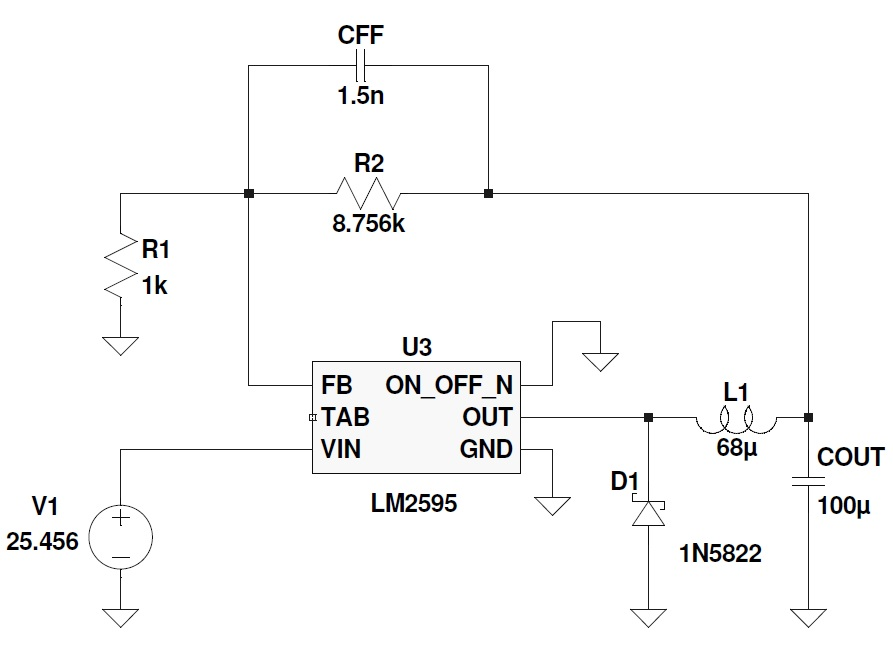
\includegraphics[width = 0.5\linewidth]{Figures/buckconverter.jpg}
        \caption{Circuit schematic of the 12V regulator}
    \label{fig:buckconvdiagram}
\end{figure}

\begin{figure}
    \centering
    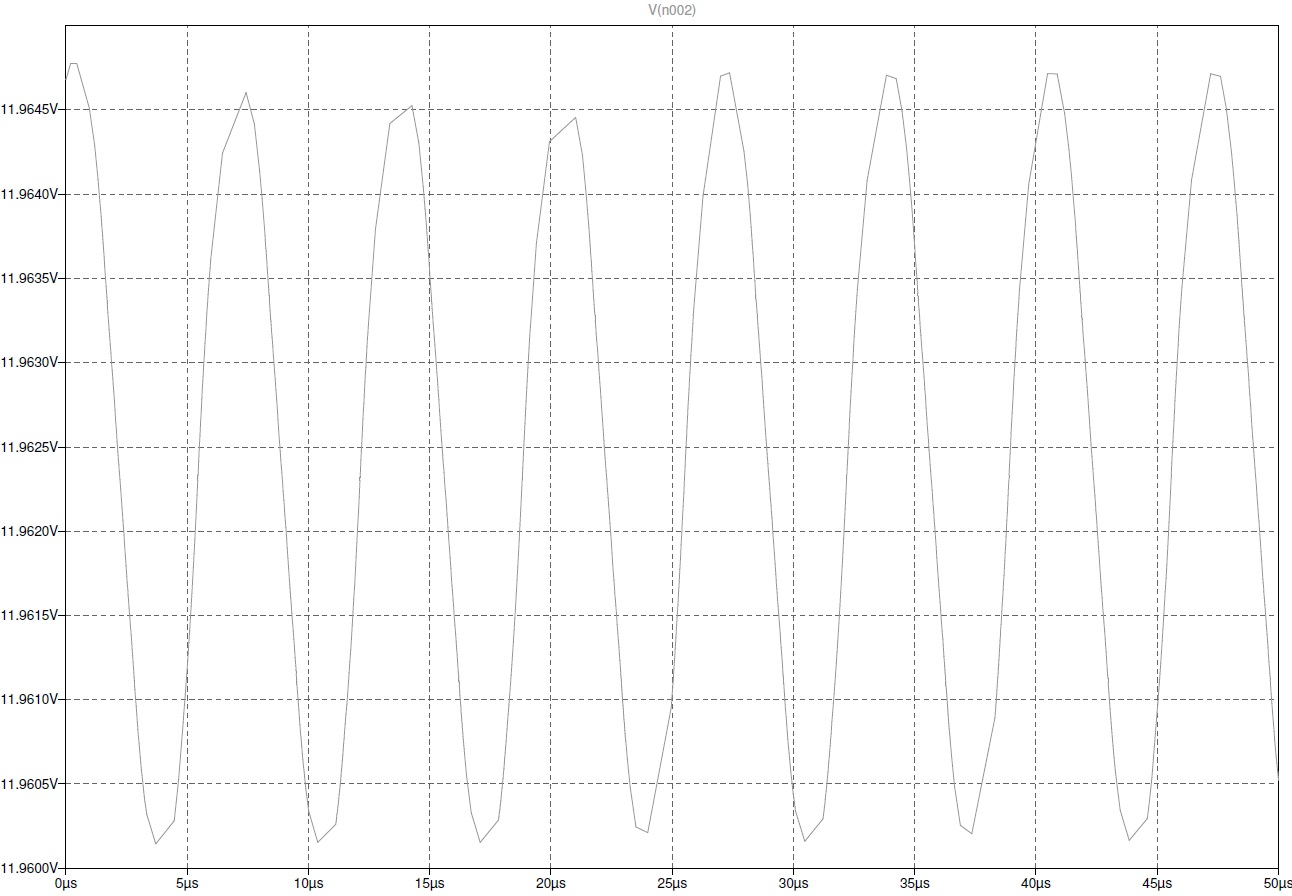
\includegraphics[width = 0.5\linewidth]{Figures/buckconverter12vplot.jpg}
    \caption{12V regulator tested with $\SI{18}{V_{RMS}}$ input}
    \label{fig:buckconvplot}
\end{figure}

\section{Measurements} \label{sec:measurements_switchmode}
After the circuit was built the output was measured and plotted using an oscilloscope as can be seen in Figure \ref{fig:buck_converter_results_box}. Using a potentiometer to adjust the resistance of $R_{2}$ the output voltage was obtained as $\SI{11.8}{V}$. The noise from the $\SI{12}{V}$ regulator was found as $\SI{61.8}{\milli V}$, which was substantially higher than the result obtained in SPICE, however there were no noise level requirements for the design of the intermediary voltage supply and thus it had no negative effects on the design of the system. 

\begin{figure}
 \centering
     \begin{subfigure}[]{0.45\textwidth}
        \centering
         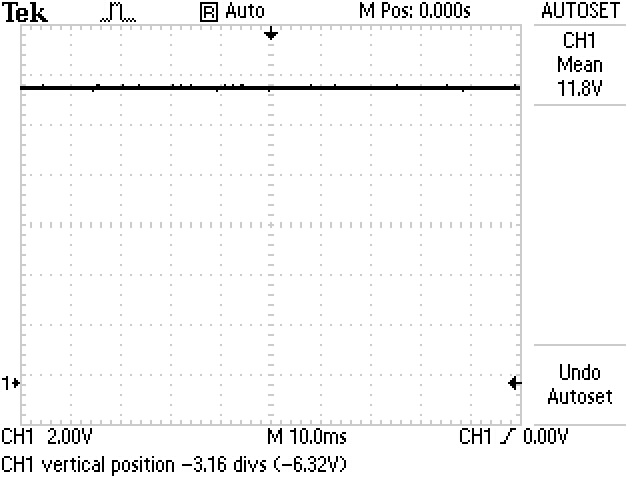
\includegraphics[width=1\linewidth]{./Figures/12V_output_voltage.JPG}
		    \caption{Buck converter output} \label{subfig:24V}
     \end{subfigure}
      \begin{subfigure}[]{0.45\textwidth}
              \centering
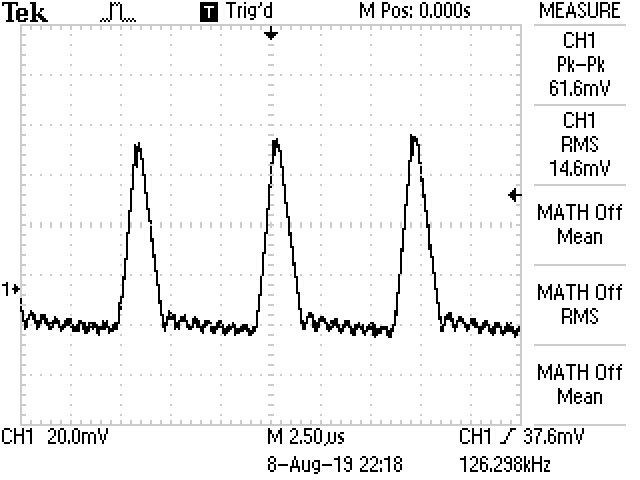
\includegraphics[width=1\linewidth]{./Figures/12V_output_noise.JPG}%
		    \caption{Noise characteristics}  \label{subfig:18V}
     \end{subfigure}
   \caption[Measured 12V Regulator Output Voltage Plots]{Measured 12V Regulator Output Voltage Plots. (a) reading showing output voltage, (b) output noise of the regulator}
    \label{fig:buck_converter_results_box}
 \end{figure}








